% !TeX root = ../tesis.tex

\section{Contraste con la literatura}
\label{section:Res_Esferocito}

Con el fin de evaluar la capacidad del modelo para reproducir resultados reportados en la literatura, se compararon las simulaciones realizadas en este trabajo con estudios numéricos y experimentales previamente publicados. En cuanto a la comparación numérica se emplearon los resultados de Tsinopoulos et al. \cite{tsinopoulosLightScatteringAggregated2002}, quienes emplearon el modelo de eritrocito propuesto por Fung \cite{fungBiomechanicsMechanicalProperties1990}, descrito por la ecuación en coordenadas cilíndricas
%
\begin{equation}
	z(\rho)=\left[1-\left(\dfrac{\rho}{a}\right)^2\right]^{1/2}\left[0.72+4.152\left(\dfrac{\rho}{a}\right)^2-3.426\left(\dfrac{\rho}{a}\right)^4\right],
	\label{eq:Tsang_eri}
\end{equation}
%
donde $a$ es el radio del eritrocito, para el cual se empleó el valor de $3.825\,\mu$m. Esta geometría corresponde a un eritrocito con un grosor mínimo de $1.44\,\mu$m y un grosor máximo de $2.84\,\mu$m, un volumen de $97.91~\mu\text{m}^3$ y un área superficial de $129.95~\mu\text{m}^2$. %
% --- JAUA ---
% Área superficies no es un pleaonasmo??
%
Cabe señalar que esta parametrización fue desarrollada para describir eritrocitos sanos, por lo que su aplicación se restringe a este tipo de células. En sus simulaciones, Tsinopoulos et al. emplearon el Método de Elementos de Frontera (BEM por sus siglas en inglés)
% --- JAUA ---
% Con CST lo pusiste en inglés y lo pusiste en itálicas
%
y consideraron un eritrocito orientado con su eje de simetría a lo largo de la dirección $z$, iluminado por una onda plana propagándose en la misma dirección y polarizada en $x$, con una longitud de onda de $632.8~\text{nm}$. En esta longitud de onda consideraron un índice de refracción de 1.402 para el eritrocito y de 1.335 para el plasma, lo que corresponde a un índice de refracción relativo de aproximadamente 1.05. Estas mismas condiciones fueron reproducidas en CST empleando los parámetros de convergencia determinados %
% --- JAUA ---
% en la Sección XX
%
\sout{previamente}. En la Fig. \ref{fig:Tsinopoulos} se muestran los resultados de la sección transversal diferencial de esparcimiento $\dd{C_{\text{sca}}/\dd{\Omega}}$ %
% --- JAUA ---
%  [Ec. \eqref{eq:XX}]
%
en función del ángulo polar $\theta$  obtenidos mediante CST con puntos azules y los obtenidos mediante BEM extraídos de la Ref.~\cite{tsinopoulosLightScatteringAggregated2002}. En la Fig. \ref{subfig:Tsi_par} se muestra el corte de $\varphi=0$, mientras que en la Fig. \ref{subfig:Tsi_perp} se muestra el corte de $\varphi=\pi/2$.
% --- JAUA ---
% Más a delante los llamas paralelo y perpendicular, pero no dices respecto a qué (suóngo que al vector de onda incidente)
%

%
\begin{figure}[h!]
	\centering
	\sidesubfloat[First image]{\hspace{-0.1cm}{
			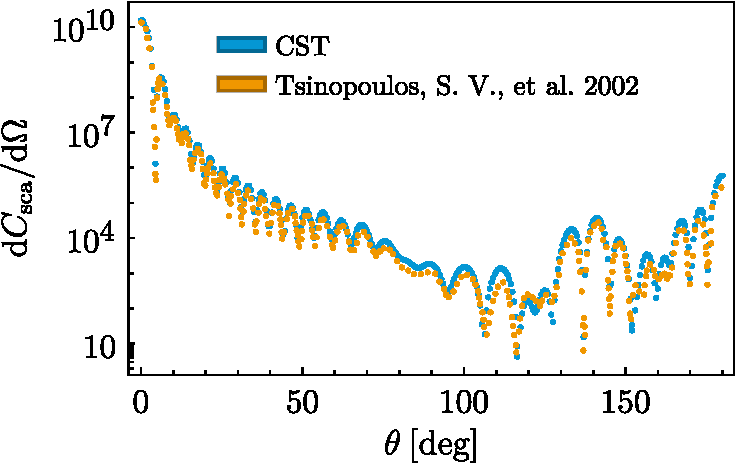
\includegraphics[width=0.45\textwidth]{../Figuras/4-Resultados/comparacionpaper0.pdf}\label{subfig:Tsi_par}}}\hspace{0.1cm}
	\sidesubfloat[Second image]{\hspace{-0.1cm}{	
\includegraphics[width=0.45\textwidth]{../Figuras/4-resultados/comparacionpaper90.pdf}\label{subfig:Tsi_perp}}}
	
	
	\caption{Sección transversal diferencial de esparcimiento $\dd{C_{\text{sca}}/\dd{\Omega}}$ en función del ángulo polar $\theta$ para un eritrocito con geometría descrita por Fung \cite{fungBiomechanicsMechanicalProperties1990} y con radio igual a 3.825 $\mu$m. El eritrocito fue iluminado por una onda plana propagándose en la dirección $z$ y polarizada en $x$, con una longitud de onda de $632.8~\text{nm}$. Se consideró un índice de refracción relativo de 1.05. Los puntos azules muestran los resultados obtenidos mediante el método FIT y los naranjas mediante BEM en la Ref.  \cite{tsinopoulosLightScatteringAggregated2002}}
	\label{fig:Tsinopoulos}
\end{figure}
%
A pesar de las diferencias observadas en la amplitud de $\dd{C_{\text{sca}}/\dd{\Omega}}$, ambos métodos reproducen la misma estructura angular general del patrón de dispersión.
% --- JAUA ---
% ChatGPT?? Nosotros le decimos esparcimiento, no? Dispersión es dependencia en omega (o en lambdas).
% Al final del párrafo también le pones así
%
En particular, en el plano paralelo ($\varphi=0$), la diferencia entre en la posición angular de los máximos locales obtenida en la Ref.~\cite{tsinopoulosLightScatteringAggregated2002} y la obtenida en CST es de $0.63^\circ$. De manera similar, en el plano perpendicular ($\varphi=\pi/2$), la diferencia promedio en la localización de los máximos locales es de  $0.46^\circ$. Estos resultados indican que el modelo implementado en CST reproduce adecuadamente el patrón angular de dispersión reportado por Tsinopoulos et al., proporcionando una validación adicional de la metodología numérica empleada en este trabajo.


% --- JAUA ---
% Esto tiene más sentido antes del análisis en del patrón de esparcimiento. Cambialo antes por favor.
%
%
Por otro lado, en la Fig. \ref{fig:Tsang_Cassini} se muestra la comparación de la geometría empleada en la Ref.~\cite{tsinopoulosLightScatteringAggregated2002} dada por la Ec. \ref{eq:Tsang_eri} (línea continua naranja) con la geometría basada en óvalos de Cassini (línea continua morada) para un eritrocito sano con los parámetros $a=2.657\,\mu$m, $b=2.75\,\mu$m y $c=1\,\mu$m. Los parámetros del óvalo de Cassini fueron seleccionados de manera que se conservaran el radio característico y espesores similares a los del modelo de Fung, obteniéndose un grosor mínimo de $1.42\,\mu$m, un grosor máximo de $2.85\,\mu$m, un volumen de $104.78~\mu\text{m}^3$ y un área superficial de $126.28~\mu\text{m}^2$. Aunque ambas geometrías presentan dimensiones comparables, se observa que el modelo de Fung exhibe una concavidad más pronunciada y bordes más afilados en la región ecuatorial.
 %
\begin{figure}[h!]
	\centering
	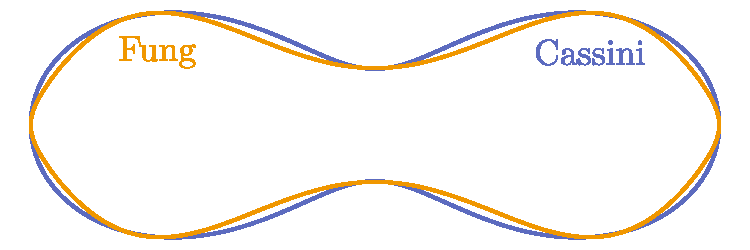
\includegraphics[width=7cm]{../../Figuras/4-Resultados/comparacion_geom_eri.pdf}
	\caption{Comparación entre el modelo de Fung dado por la Ec. \ref{eq:Tsang_eri} y el modelo de óvalos de Cassini, dado po la Ec. \ref{eq:cassini} con valores de $a=2.657\,\mu$m, $b=2.75\,\mu$m y $c=1\,\mu$m. }
	\label{fig:Tsang_Cassini}
\end{figure}
%

**REVISAR HASTA AQUÍ**


En la Fig. se muestran las diferencias entre $\dd{C_{\text{sca}}/\dd{\Omega}}$ en función del ángulo polar $\theta$  obtenidos empleando la geometría de óvalos de Cassini con puntos morados y la de Tsang con puntos naranja. Se observa que 
%
\begin{figure}[h!]
	\centering
	\sidesubfloat[First image]{\hspace{-0.1cm}{
			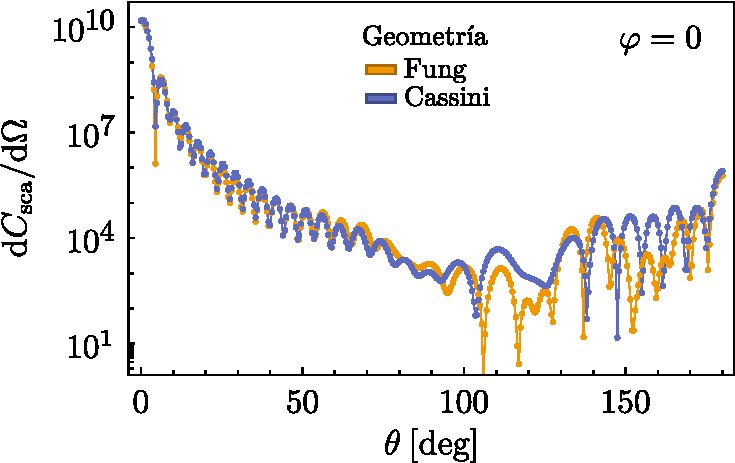
\includegraphics[width=0.45\textwidth]{../Figuras/4-Resultados/comparacionpaperCassini0.pdf}\label{subfig:Fung_Cass_par}}}\hspace{0.1cm}
	\sidesubfloat[Second image]{\hspace{-0.1cm}{	
\includegraphics[width=0.45\textwidth]{../Figuras/4-resultados/comparacionpaperCassini90.pdf}\label{subfig:Fung_Cass_perp}}}
	
	
	\caption{Sección transversal diferencial de esparcimiento $\dd{C_{\text{sca}}/\dd{\Omega}}$ en función del ángulo polar $\theta$ para un eritrocito con geometría descrita por Fung \cite{fungBiomechanicsMechanicalProperties1990} (puntos naranjas) y para un eritrocito con geometría descrita por óvalos de Cassini con $a=2,657$ nm, $b=2750$ nm y $c=1000$ nm. En ambos casos el eritrocito fue iluminado por una onda plana propagándose en la dirección $z$ y polarizada en $x$, con una longitud de onda de $632.8~\text{nm}$. Se consideró un índice de refracción relativo de 1.05.}
	\label{fig:Tsinopoulos}
\end{figure}
%



*FALTA ESCRIBIR LO DEL PAPER EXPERIMENTAL*
